\chapter{Intercambio respiratorio de gases}\label{ch:b1:gas-exchange}

Un litro de aire contiene treinta veces más oxígeno que un litro de agua,
pesa ochocientas veces menos y deja que el oxígeno difunda por él diez mil
veces más deprisa. Una trucha debe hacer pasar ciento cincuenta gramos de
agua por sus \omterm{def:b1:gas-exchange:gill}{branquias} por cada miligramo de oxígeno que toma, y extrae
cuatro quintas partes de lo que el agua transporta; un ser humano mueve unos
pocos gramos de aire por miligramo y desperdicia tres cuartas partes. Los
dos \omterm{def:b1:mammal-organization:organ}{órganos} son respuestas a la misma ecuación --- el flujo de un gas a
través de una superficie --- en dos medios. Este capítulo enuncia la física,
deduce cómo debe ser una \omterm{prop:b1:organism-environment:surfaces}{superficie de intercambio}, describe \omterm{def:b1:gas-exchange:gill}{branquias},
pulmones y tráqueas, sigue el oxígeno y el dióxido de carbono por la sangre,
y observa cómo se controla la ventilación y qué cambia en altitud y bajo el
agua.

\section{La física de un gas en dos medios}

\begin{definition}[Presión parcial, solubilidad]\label{def:b1:gas-exchange:partial}
\index{presión parcial}
En una mezcla de gases, cada gas ejerce una \emph{presión parcial}
proporcional a su fracción: en aire a \qty{101}{kPa}, el oxígeno
(\qty{20.9}{\%}) tiene $P_{\mathrm{O_2}} = \qty{21.2}{kPa}$, y el dióxido de
carbono (\qty{0.04}{\%}), \qty{0.04}{kPa}. Un gas se disuelve en un líquido
en proporción a su presión parcial (ley de Henry): el agua en equilibrio con
el aire a \qty{15}{\celsius} contiene \qty{0.32}{mmol/L} de oxígeno
(\qty{10}{mg/L}, \qty{7}{mL/L} de gas), frente a \qty{8.7}{mmol/L}
(\qty{210}{mL/L}) en el propio aire. La presión parcial --- la misma en el
agua y en el aire cuando están en equilibrio --- es lo que impulsa la
difusión entre medios; el contenido es lo que un ser que respira puede
extraer. El dióxido de carbono es veinticinco veces más soluble que el
oxígeno, de modo que nunca es el gas más difícil de intercambiar.
\end{definition}

\begin{theorem}[Ley de Fick para una superficie de intercambio]\label{thm:b1:gas-exchange:fick}
\index{ley de Fick}
La velocidad a la que un gas atraviesa una membrana de área $A$ y espesor
$x$ que separa dos medios a las presiones parciales $P_1$ y $P_2$ es
\[
\dot V = K\,\frac{A}{x}\,(P_1 - P_2),
\]
donde $K$, la constante de difusión (de Krogh) de la membrana, engloba la
difusividad y la solubilidad del gas en el \omterm{def:b1:body-plans-tissues:tissue}{tejido}. El flujo lo eleva un área
mayor, una barrera más delgada y una diferencia mayor de \omterm{def:b1:gas-exchange:partial}{presión parcial};
nada más.
\end{theorem}
\begin{proof}
La primera \omterm{thm:b1:membranes-transport:fick}{ley de Fick} para el gas disuelto en la membrana
(\cref{ch:b1:membranes-transport}) da un flujo por unidad de área
proporcional al gradiente de concentración; por la ley de Henry, la
concentración en cada cara es proporcional a la \omterm{def:b1:gas-exchange:partial}{presión parcial} del medio de
ese lado, así que el gradiente es $(P_1 - P_2)/x$ por la solubilidad, y la
constante absorbe la solubilidad y la difusividad.
\end{proof}

\begin{omfigure}
\begin{tikzpicture}
\begin{axis}[
  ybar, bar width=16pt,
  width=0.72\linewidth, height=5.6cm,
  axis x line=bottom, axis y line=left,
  ymode=log, log origin=infty, ymin=0.1, ymax=3000,
  ylabel={oxígeno por litro de medio (\unit{mL})},
  ylabel style={font=\small},
  symbolic x coords={aire, agua a 5 C, agua a 15 C, agua a 30 C, agua de mar a 15 C},
  xtick=data, x tick label style={font=\small, rotate=20, anchor=north east},
  enlarge x limits=0.15,
  nodes near coords, nodes near coords style={font=\scriptsize, anchor=south},
  point meta=rawy,
]
\addplot[fill=omDef!45, draw=omDef] coordinates {(aire,210) (agua a 5 C,9.0) (agua a 15 C,7.1) (agua a 30 C,5.3) (agua de mar a 15 C,5.8)};
\end{axis}
\end{tikzpicture}

{\small Contenido de oxígeno del aire y del agua en equilibrio con él. El
agua contiene treinta veces menos, y todavía menos cuando está caliente o
salada: un pez en una charca de verano vive al borde del suministro.}
\end{omfigure}

\begin{proposition}[Cómo debe ser una superficie de intercambio]\label{prop:b1:gas-exchange:requirements}
\index{superficie de intercambio}
Un \omterm{def:b1:organism-environment:organism}{organismo} de más de un milímetro no puede abastecerse por difusión a
través de su superficie externa (\cref{ch:b1:organism-environment}).
Necesita una \emph{superficie respiratoria} que sea grande (para elevar
$A$), delgada (para reducir $x$), húmeda (los gases solo atraviesan las
membranas en disolución), \emph{ventilada} --- con el medio exterior
renovado, para que $P_1$ se mantenga alta --- y \emph{perfundida} --- con la
sangre de detrás renovada, para que $P_2$ se mantenga baja ---; y una
circulación que lleve el gas desde la superficie hasta los \omterm{def:b1:body-plans-tissues:tissue}{tejidos}. Las
\omterm{def:b1:gas-exchange:gill}{branquias}, los pulmones y las tráqueas son tres maneras de plegar una
superficie así dentro de un cuerpo y de hacer pasar los dos fluidos por
ella.
\end{proposition}

\section{Las branquias y la contracorriente}

\begin{definition}[Branquia]\label{def:b1:gas-exchange:gill}
\index{branquia}
Una \emph{branquia} es una evaginación de la superficie corporal hacia el
agua, plegada en filamentos y \emph{laminillas} de unos micrómetros de
espesor por los que la sangre circula en capilares. Las branquias de un pez
cuelgan de cuatro arcos óseos a cada lado; el agua, que entra por la boca y
sale por debajo de los opérculos gracias a un sistema de dos bombas, fluye
entre las laminillas en un sentido, y la sangre de las laminillas fluye en
el contrario: una \emph{contracorriente}\index{intercambio a contracorriente}. Una trucha de un kilogramo tiene unos \qty{2000}{cm^2} de
superficie laminar, de \qty{2}{\micro m} de espesor.
\end{definition}

\begin{omfigure}
\begin{tikzpicture}
  \node[anchor=south west, inner sep=0] (img) at (0,0)
    {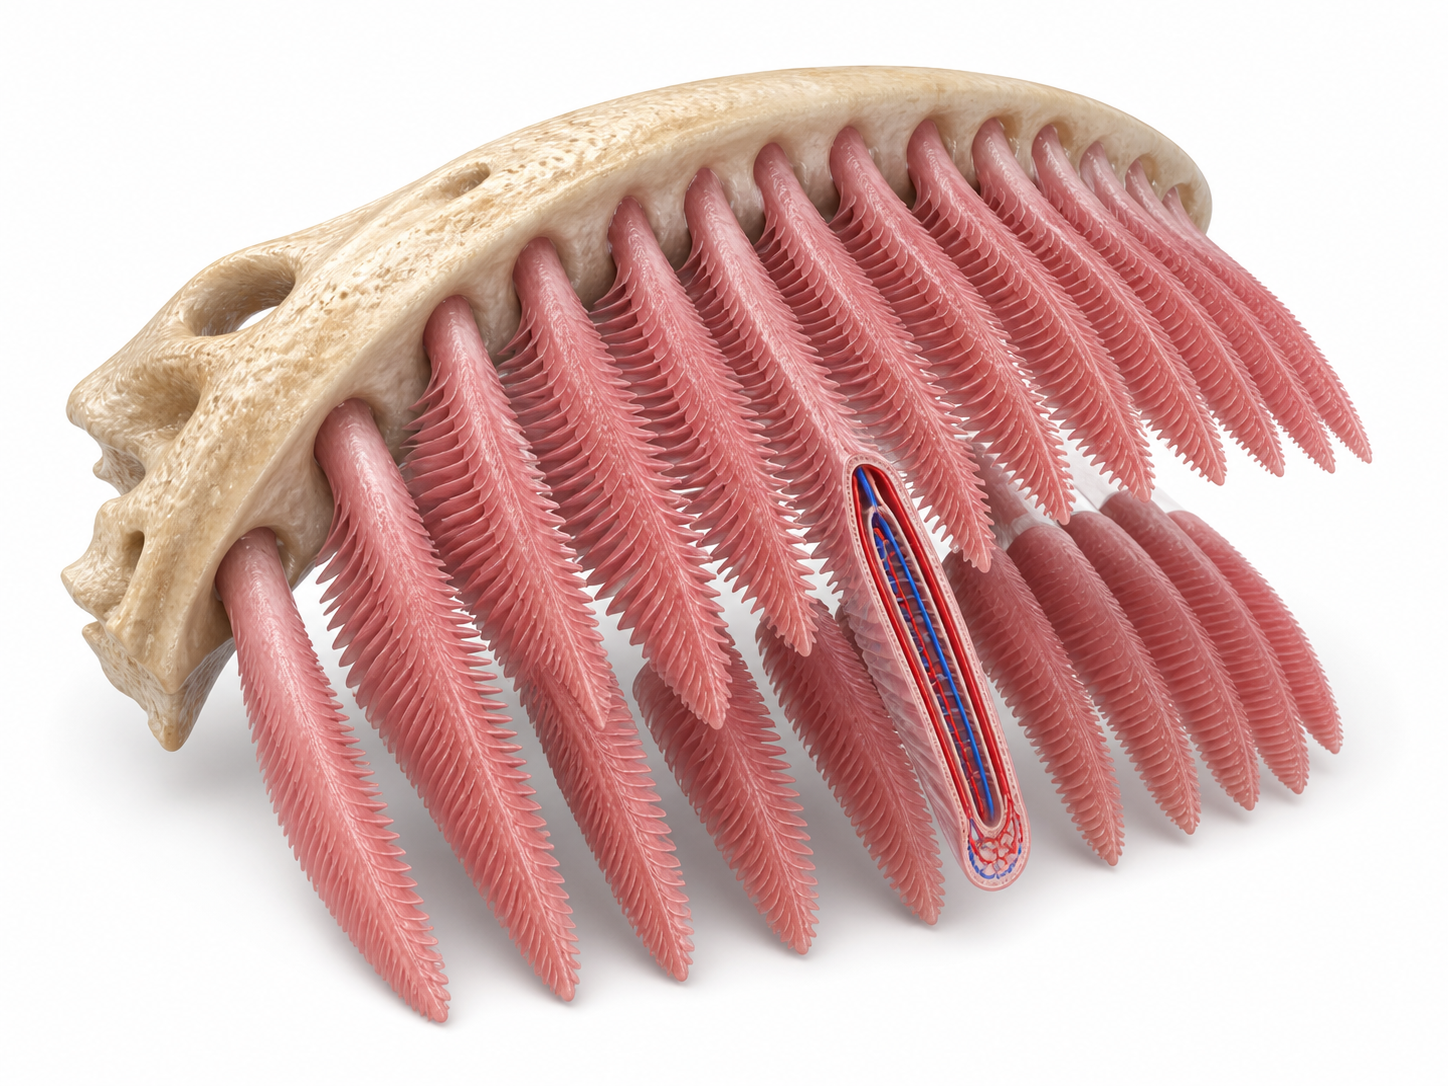
\includegraphics[width=0.52\linewidth]{images/book3/ai/fig-gill-lamellae.png}};
  \begin{scope}[x={(img.south east)}, y={(img.north west)},
      every node/.style={font=\small}]
    \draw[omDef, thick] (0.20,0.50) -- (-0.03,0.60) node[left] {arco branquial};
    \draw[omDef, thick] (0.55,0.70) -- (0.55,1.08) node[above] {filamentos};
    \draw[omDef, thick] (0.75,0.40) -- (1.03,0.30) node[right, align=left] {laminillas: la superficie de\\ intercambio, \qty{2}{\micro m} de espesor};
    \draw[omDef, thick] (0.45,0.20) -- (0.45,-0.08) node[below] {vasos sanguíneos a lo largo del filamento};
  \end{scope}
\end{tikzpicture}

{\small Un arco branquial con sus filamentos y sus laminillas. El agua fluye
entre las laminillas; la sangre las atraviesa en sentido contrario.}
\end{omfigure}

\begin{theorem}[Intercambio a contracorriente]\label{thm:b1:gas-exchange:countercurrent}
Cuando el agua y la sangre fluyen en sentidos opuestos a lo largo de una
\omterm{prop:b1:organism-environment:surfaces}{superficie de intercambio}, la sangre que sale de la \omterm{def:b1:gas-exchange:gill}{branquia} puede acercarse
a la \omterm{def:b1:gas-exchange:partial}{presión parcial} del agua que \emph{entra} en ella, y el agua puede
quedar despojada de casi todo su oxígeno: extracciones del \qty{80}{\%} o
más. Cuando fluyen en el mismo sentido (a favor de corriente), ambos fluidos
convergen a un valor intermedio común y la extracción no puede superar el
\qty{50}{\%}.
\end{theorem}
\begin{proof}
A lo largo de un intercambiador a favor de corriente, la diferencia
$P_{\text{agua}} -
P_{\text{sangre}}$ cae desde su valor de entrada hasta
cero a medida que ambos se acercan a la misma presión; una vez iguales, ya
no se mueve más gas, y con caudales iguales el punto de encuentro está a
mitad de camino. En la \omterm{def:b1:gas-exchange:gill}{contracorriente}, la sangre, conforme avanza hacia su
salida, se encuentra con agua cada vez más fresca, de modo que se mantiene
una diferencia positiva a lo largo de toda la longitud; la sangre de la
salida se enfrenta al agua entrante a \qty{21}{kPa}, y el agua de la salida
se enfrenta a la sangre venosa entrante, a unos pocos kilopascales. El
límite lo fija la superficie, no un equilibrio.
\end{proof}

\begin{omfigure}
\begin{tikzpicture}[font=\footnotesize, >=Stealth, line cap=round]
  % co-current
  \begin{scope}
    \node[anchor=south, font=\small] at (2.6,1.65) {a favor de corriente: ambos flujos en el mismo sentido};
    \draw[->, very thick, omDef] (0,1.2) -- (5.2,1.2) node[right] {sale agua: \qty{12}{kPa}};
    \draw[->, very thick, omThm] (0,0.4) -- (5.2,0.4) node[right] {sale sangre: \qty{12}{kPa}};
    \node[anchor=east, omDef] at (-0.1,1.2) {entra agua: \qty{21}{kPa}};
    \node[anchor=east, omThm] at (-0.1,0.4) {entra sangre: \qty{3}{kPa}};
    \foreach \x/\d in {0.6/18, 1.6/12, 2.6/7, 3.6/3, 4.6/0.5} { \draw[->, gray] (\x,1.05) -- (\x,0.55) node[midway, right, font=\scriptsize, gray] {\d}; }
    \node[anchor=north, align=center] at (2.6,0.1) {la diferencia (gris, kPa) se reduce a cero:\\ la extracción se detiene en el \qty{43}{\%}};
  \end{scope}
  \begin{scope}[yshift=-3.6cm]
    \node[anchor=south, font=\small] at (2.6,1.65) {contracorriente: flujos opuestos};
    \draw[->, very thick, omDef] (0,1.2) -- (5.2,1.2) node[right] {sale agua: \qty{4}{kPa}};
    \draw[<-, very thick, omThm] (0,0.4) -- (5.2,0.4) node[right] {entra sangre: \qty{3}{kPa}};
    \node[anchor=east, omDef] at (-0.1,1.2) {entra agua: \qty{21}{kPa}};
    \node[anchor=east, omThm] at (-0.1,0.4) {sale sangre: \qty{18}{kPa}};
    \foreach \x/\d in {0.6/3, 1.6/3, 2.6/3, 3.6/3, 4.6/2} { \draw[->, gray] (\x,1.05) -- (\x,0.55) node[midway, right, font=\scriptsize, gray] {\d}; }
    \node[anchor=north, align=center] at (2.6,0.1) {la diferencia sigue siendo positiva en todo el trayecto:\\ la extracción llega al \qty{80}{\%} y la sangre sale cerca del valor de entrada del agua};
  \end{scope}
\end{tikzpicture}

{\small Intercambio a favor de corriente y a \omterm{def:b1:gas-exchange:gill}{contracorriente} con la misma
superficie y los mismos caudales. Oponer los flujos mantiene un gradiente en
toda la longitud y permite que la sangre se acerque a la presión de oxígeno
del agua fresca.}
\end{omfigure}

\begin{omfigure}
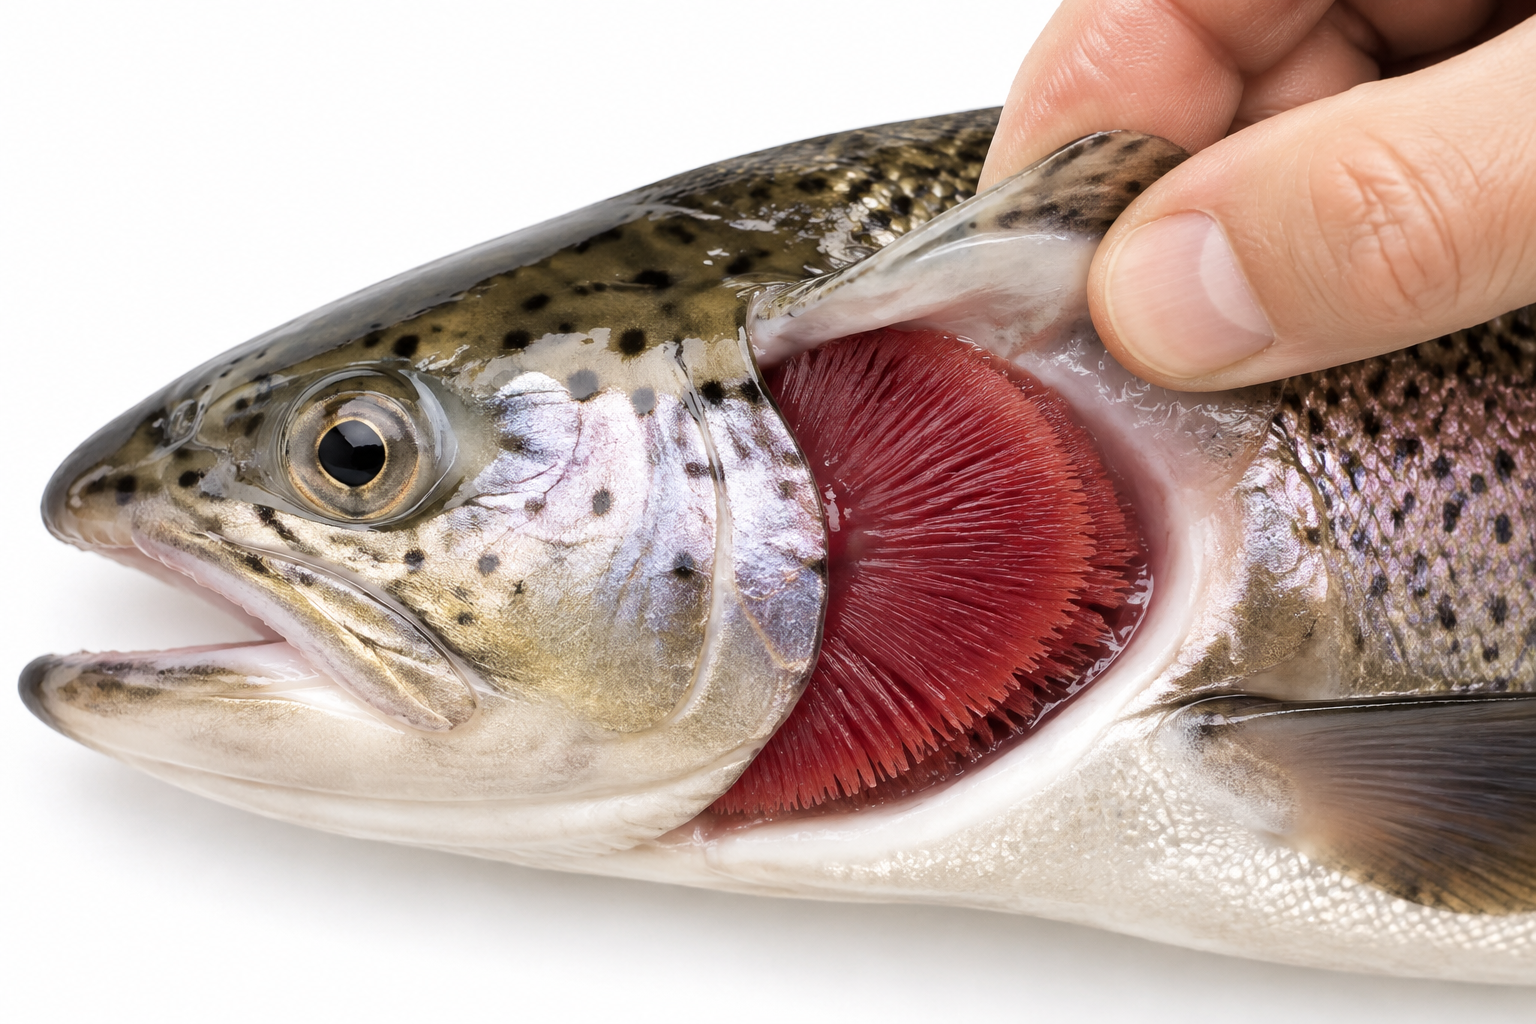
\includegraphics[width=0.5\linewidth]{images/book3/ai/b3-21-trout-gills.png}

{\small Las \omterm{def:b1:gas-exchange:gill}{branquias} de una trucha bajo el opérculo levantado: rojas de
sangre, porque las laminillas tienen dos \omterm{def:b1:cell-unit-of-life:cell}{células} de espesor y la sangre está
a un micrómetro del agua.}
\end{omfigure}

\begin{example}[El precio del agua]\label{ex:b1:gas-exchange:priceofwater}
Una trucha de \qty{1}{kg} en reposo toma unos \qty{50}{mL} de oxígeno por
hora. De un agua con \qty{7}{mL/L}, y con un \qty{80}{\%} de extracción,
debe bombear \qty{9}{L} de agua por hora a través de sus \omterm{def:b1:gas-exchange:gill}{branquias}: nueve
kilogramos de un medio cincuenta veces más viscoso que el aire, por \omterm{def:b1:membranes-transport:transporters}{canales}
de una fracción de milímetro de ancho. Una décima parte de su metabolismo se
va en respirar; un ser humano en reposo gasta una cincuentava. Caliéntese la
charca a \qty{30}{\celsius} y ese mismo pez, que necesita más oxígeno de un
agua que contiene menos, deberá bombear el triple.
\end{example}

\section{Respirar aire: pulmones y tráqueas}

\begin{definition}[El pulmón de los mamíferos]\label{def:b1:gas-exchange:lung}
\index{pulmón}\index{alvéolo}
Un \emph{pulmón} es una invaginación de la superficie corporal hacia una
cámara interna húmeda, lo que mantiene mojada la superficie en aire seco. El
pulmón de los mamíferos es un árbol de vías aéreas que termina en unos
trescientos millones de \emph{alvéolos}, sáculos de \qty{0.2}{mm} de
diámetro cuyas paredes --- una \omterm{def:b1:cell-unit-of-life:cell}{célula} epitelial y un endotelio capilar,
\qty{0.5}{\micro m} en total --- suman \qty{100}{m^2} en un ser humano,
envueltas en una red capilar por la que pasa todo el gasto cardíaco. Se
ventila de forma \emph{mareal}: el \omterm{def:b1:mammal-organization:bodyplan}{diafragma} y los músculos costales
agrandan el tórax y entra aire; se relajan y el aire sale por el mismo
camino. Una respiración mueve \qty{500}{mL}, de los que \qty{150}{mL} solo
llenan las vías aéreas (el \emph{espacio muerto}) y nunca llegan a un
alvéolo; el gas alveolar, renovado en una séptima parte en cada respiración,
se mantiene a $P_{\mathrm{O_2}} =
\qty{13.3}{kPa}$ y
$P_{\mathrm{CO_2}} = \qty{5.3}{kPa}$: las presiones con las que se equilibra
la sangre.
\end{definition}

\begin{omfigure}
\begin{tikzpicture}
  \node[anchor=south west, inner sep=0] (img) at (0,0)
    {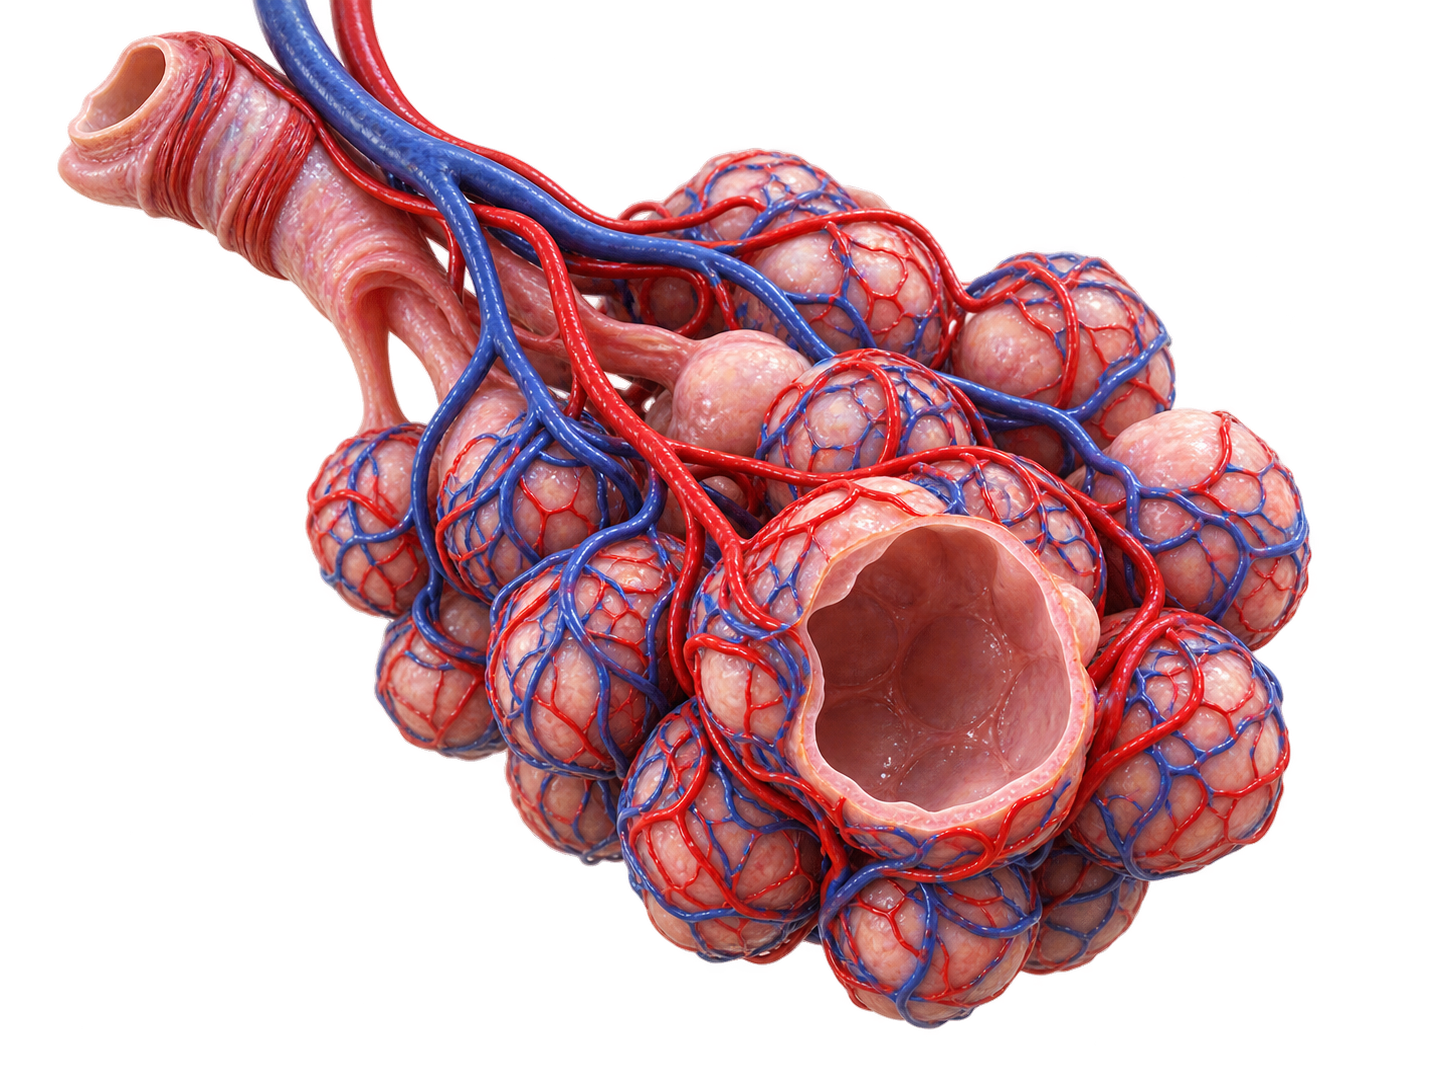
\includegraphics[width=0.5\linewidth]{images/book3/ai/fig-alveoli.png}};
  \begin{scope}[x={(img.south east)}, y={(img.north west)},
      every node/.style={font=\small}]
    \draw[omDef, thick] (0.50,0.85) -- (0.50,1.08) node[above] {vía aérea terminal};
    \draw[omDef, thick] (0.30,0.45) -- (-0.03,0.40) node[left, align=right] {alvéolo abierto:\\ aire dentro};
    \draw[omDef, thick] (0.75,0.55) -- (1.03,0.62) node[right, align=left] {red capilar\\ sobre la pared};
    \draw[omDef, thick] (0.60,0.15) -- (0.60,-0.08) node[below] {pared: \qty{0.5}{\micro m} entre el aire y la sangre};
  \end{scope}
\end{tikzpicture}

{\small \omterm{def:b1:gas-exchange:lung}{Alvéolos} al final de una vía aérea, envueltos en capilares. Todo el
gasto cardíaco se extiende sobre cien metros cuadrados de esta pared, una
fracción de segundo cada vez.}
\end{omfigure}

\begin{proposition}[Tres diseños para el aire]\label{prop:b1:gas-exchange:designs}
\index{tráqueas}
Los \emph{mamíferos} ventilan de forma mareal: es sencillo, pero el aire
fresco se mezcla con el viciado, el oxígeno alveolar es dos tercios del
atmosférico y la extracción es de una cuarta parte. Las \emph{aves} hacen
pasar el aire en un solo sentido por tubos finos (parabronquios) situados
entre dos juegos de sacos aéreos que actúan como fuelles, de modo que el
aire fresco atraviesa la \omterm{prop:b1:organism-environment:surfaces}{superficie de intercambio} tanto en la inspiración
como en la espiración, en corriente cruzada con la sangre: su extracción es
mayor, y un ánsar indio vuela sobre el Himalaya donde un mamífero se
desmayaría. Los \emph{insectos} no tienen sangre respiratoria en absoluto:
el aire entra por unas válvulas (los \emph{espiráculos}) hacia unas
\emph{tráqueas}, tubos rigidizados por engrosamientos en espiral que se
ramifican hasta el micrómetro y entregan el oxígeno por difusión
directamente a cada \omterm{def:b1:cell-unit-of-life:cell}{célula}, con ayuda del bombeo del abdomen en los insectos
grandes o activos. La difusión a lo largo de tubos limita el diseño a
cuerpos pequeños, que es una de las razones de que ningún insecto sea mayor
que un ratón.
\end{proposition}

\begin{omfigure}
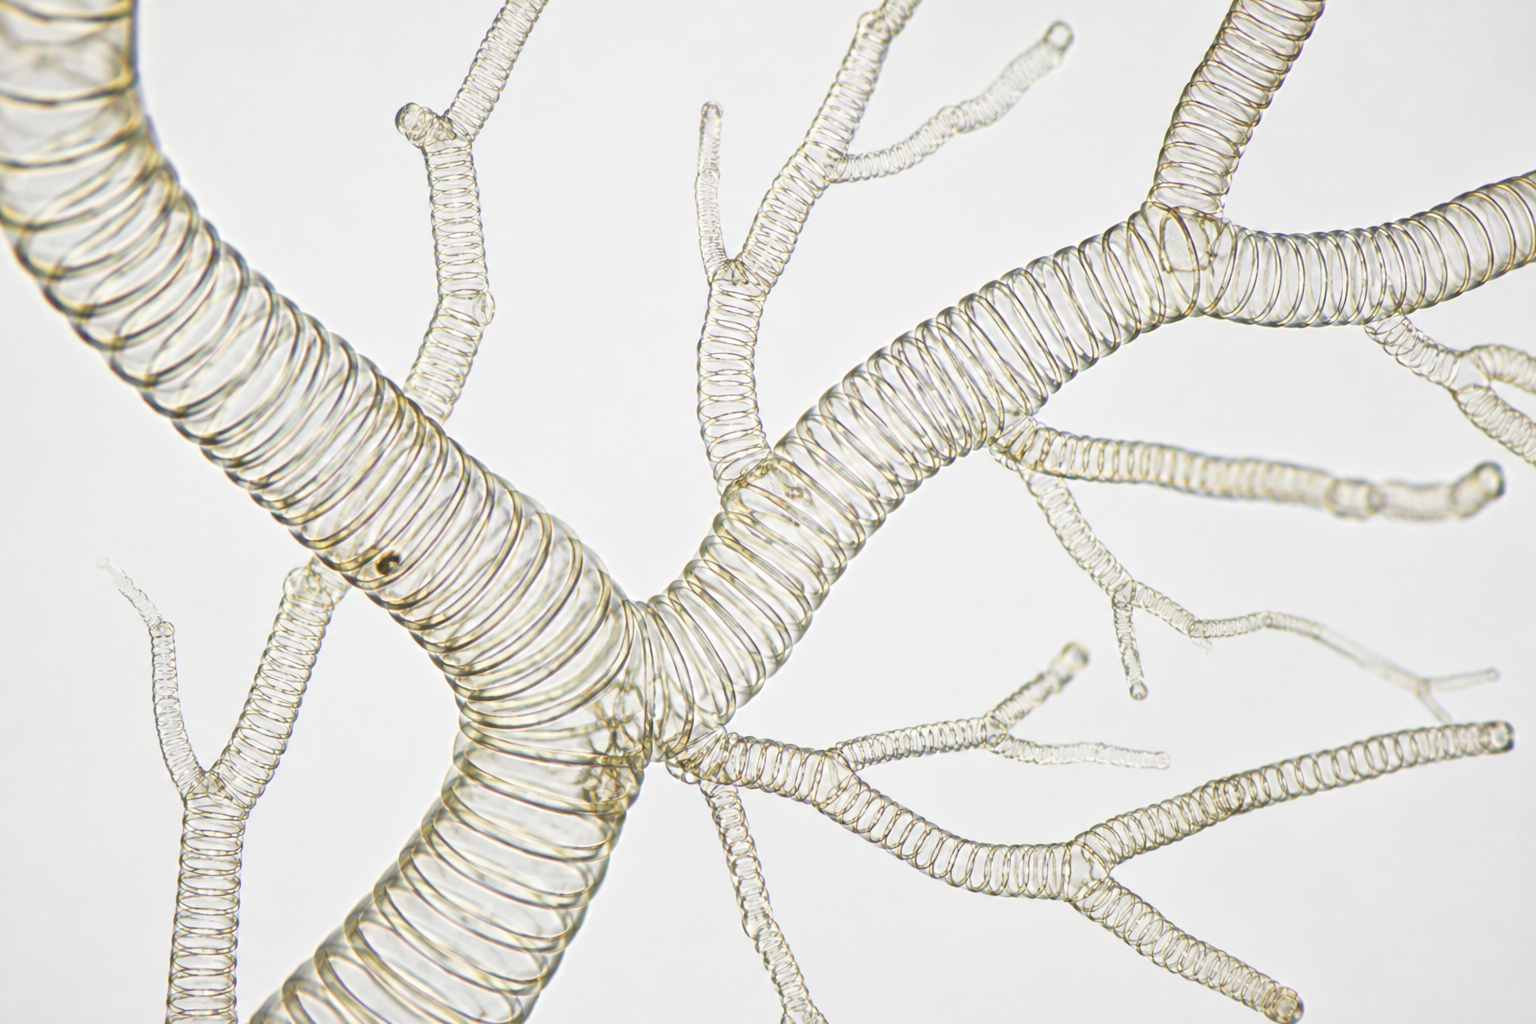
\includegraphics[width=0.5\linewidth]{images/book3/ai/b3-21-insect-tracheae.png}

{\small Tráqueas de insecto: tubos llenos de aire mantenidos abiertos por
engrosamientos en espiral, que se ramifican hasta las \omterm{def:b1:cell-unit-of-life:cell}{células}. Ninguna
sangre transporta el oxígeno; el aire llega hasta el final.}
\end{omfigure}

\begin{method}[Lectura de un balance de ventilación]\label{met:b1:gas-exchange:budget}
\begin{enumerate}
  \item Ventilación por minuto $=$ volumen corriente $\times$ respiraciones
        por minuto; ventilación alveolar $=$ (volumen corriente $-$ espacio
        muerto) $\times$ respiraciones por minuto. Solo la segunda
        intercambia gas.
  \item Captación de oxígeno $=$ ventilación alveolar $\times$ (fracción
        inspirada $-$ fracción alveolar); en reposo,
        $\qty{4.2}{L/min}\times(0.21 - 0.14) \approx \qty{0.3}{L/min}$.
  \item Extracción $=$ captación $/$ (ventilación $\times$ fracción
        inspirada): una cuarta parte en un \omterm{def:b1:gas-exchange:lung}{pulmón} mareal, cuatro quintas en
        una \omterm{def:b1:gas-exchange:gill}{branquia} a \omterm{def:b1:gas-exchange:gill}{contracorriente}.
  \item Del lado de la sangre: captación $=$ gasto cardíaco $\times$
        (contenido arterial $-$ venoso); \qty{5}{L/min}$\times$
        \qty{50}{mL/L} en reposo, los mismos \qty{250}{mL/min}. Los dos
        balances deben coincidir.
\end{enumerate}
\end{method}

\section{Los gases en la sangre}

\begin{proposition}[Transporte de oxígeno y de dióxido de carbono]\label{prop:b1:gas-exchange:transport}
\index{anhidrasa carbónica}\index{efecto Bohr}\index{efecto Haldane}
El \omterm{def:b1:mammal-organization:compartments}{plasma} disuelve solo \qty{3}{mL} de oxígeno por litro a la presión
arterial; la hemoglobina (\cref{ch:b1:proteins}) transporta \qty{200}{mL},
que carga en el \omterm{def:b1:gas-exchange:lung}{pulmón} a \qty{13.3}{kPa} y descarga entre una quinta parte y
la mitad en los \omterm{def:b1:body-plans-tissues:tissue}{tejidos}. El dióxido de carbono viaja de tres maneras: un
\qty{7}{\%} disuelto, un \qty{23}{\%} unido a los grupos amino de la
hemoglobina y un \qty{70}{\%} como bicarbonato: en el glóbulo rojo, la
\emph{\omterm{prop:b1:gas-exchange:transport}{anhidrasa carbónica}} convierte el $\mathrm{CO_2}$ y el agua en ácido
carbónico en cuestión de milisegundos, el ácido se disocia, el bicarbonato
sale de la \omterm{def:b1:cell-unit-of-life:cell}{célula} a cambio de cloruro (el \emph{desplazamiento del cloruro})
y la hemoglobina capta el protón. Los dos gases se ayudan mutuamente: el
ácido y el $\mathrm{CO_2}$ rebajan la afinidad de la hemoglobina por el
oxígeno (\emph{\omterm{prop:b1:gas-exchange:transport}{efecto Bohr}}), de modo que el oxígeno se libera allí donde se
produce $\mathrm{CO_2}$; y la hemoglobina desoxigenada fija mejor los
protones y el $\mathrm{CO_2}$ (\emph{\omterm{prop:b1:gas-exchange:transport}{efecto Haldane}}), de modo que el
$\mathrm{CO_2}$ se capta allí donde se libera oxígeno, y se cede en el
\omterm{def:b1:gas-exchange:lung}{pulmón} a medida que se carga el oxígeno.
\end{proposition}

\begin{omfigure}
\begin{tikzpicture}[font=\footnotesize, >=Stealth, line cap=round]
  % red cell
  \draw[very thick, omThm!80!black, fill=omThm!8, rounded corners=18pt] (0,0) rectangle (7.6,4.0);
  \node[anchor=north west, omThm!80!black, font=\small] at (0.15,3.95) {glóbulo rojo (en un capilar de un tejido)};
  % CO2 in from tissue
  \draw[->, very thick, omDef] (-1.6,2.6) -- (0,2.6) node[pos=0, left, align=right] {$\mathrm{CO_2}$ desde\\ el tejido};
  \node[draw, thick, fill=white, rounded corners=3pt, inner sep=2pt] (ca) at (2.0,2.6) {$\mathrm{CO_2} + \mathrm{H_2O} \to \mathrm{H_2CO_3}$};
  \node[anchor=south, font=\scriptsize, omProp!80!black] at (2.0,2.95) {anhidrasa carbónica};
  \node[draw, thick, fill=white, rounded corners=3pt, inner sep=2pt] (dis) at (5.2,2.6) {$\mathrm{H^+} + \mathrm{HCO_3^-}$};
  \draw[->, thick] (ca) -- (dis);
  % bicarbonate out, chloride in
  \draw[->, very thick, omDef] (6.2,2.4) -- (6.2,0.9) -- (8.4,0.9) node[right, align=left] {$\mathrm{HCO_3^-}$ hacia el plasma\\ (\qty{70}{\%} del $\mathrm{CO_2}$)};
  \draw[<-, very thick, gray] (6.9,1.85) -- (8.4,1.85) node[right, gray] {$\mathrm{Cl^-}$ a cambio};
  % proton to Hb, O2 release
  \node[draw, thick, fill=omThm!25, rounded corners=3pt, inner sep=2pt] (hb) at (4.0,1.0) {hemoglobina};
  \draw[->, thick] (4.7,2.35) -- (4.2,1.3) node[midway, right, font=\scriptsize] {$\mathrm{H^+}$ fijado};
  \draw[->, very thick, omExo!70!black] (hb.west) -- (0,1.0) -- (-1.6,1.0) node[left, align=right] {$\mathrm{O_2}$ liberado\\ (efecto Bohr)};
  \node[anchor=north, align=center, gray] at (3.8,-0.2) {en el pulmón todas las flechas se invierten: el oxígeno se carga, los protones y el $\mathrm{CO_2}$ se liberan,\\ el bicarbonato vuelve a entrar en la célula y el $\mathrm{CO_2}$ se exhala};
\end{tikzpicture}

{\small El dióxido de carbono en un glóbulo rojo. La \omterm{prop:b1:gas-exchange:transport}{anhidrasa carbónica}
fabrica ácido carbónico; el bicarbonato sale al \omterm{def:b1:mammal-organization:compartments}{plasma} y la hemoglobina
capta el protón, y libera oxígeno al fijarlo.}
\end{omfigure}

\begin{example}[Un litro de sangre por un músculo que trabaja]\label{ex:b1:gas-exchange:litre}
La sangre arterial trae \qty{200}{mL} de oxígeno por litro y \qty{480}{mL}
de dióxido de carbono (sobre todo como bicarbonato). En un músculo en reposo
deja \qty{50}{mL} de oxígeno y capta \qty{40}{mL} de $\mathrm{CO_2}$; el pH
venoso solo baja \qty{0.04}{}, porque la hemoglobina ha absorbido los
protones. En un músculo que esprinta, a pH 7,2 y con un
$P_{\mathrm{O_2}}$ de \qty{2.7}{kPa}, ese mismo litro deja \qty{150}{mL} de
oxígeno (\cref{ch:b1:proteins}) y se lleva además el lactato.
\end{example}

\section{Control, altitud y buceo}

\begin{proposition}[La ventilación la controla el dióxido de carbono]\label{prop:b1:gas-exchange:control}
\index{quimiorreceptor}
El ritmo de la respiración se genera en el tronco encefálico y lo ajustan
los \emph{quimiorreceptores}: los centrales, bañados por el líquido que
rodea el encéfalo, responden al cambio de pH que produce el
$\mathrm{CO_2}$; los periféricos, en las arterias carótidas, responden a una
caída del oxígeno arterial por debajo de unos \qty{8}{kPa}. En la vida
ordinaria manda el $\mathrm{CO_2}$: una subida de \qty{1}{kPa} en la
$P_{\mathrm{CO_2}}$ arterial duplica aproximadamente la ventilación,
mientras que el oxígeno debe caer un tercio antes de que la ventilación
responda. Aguantar la respiración termina cuando el $\mathrm{CO_2}$, y no el
oxígeno, alcanza el límite; hiperventilar antes rebaja el $\mathrm{CO_2}$ y
permite a un buceador quedarse abajo hasta que se le agota el oxígeno:
inconsciente antes de que vuelva el impulso de respirar.
\end{proposition}

\begin{omfigure}
\begin{tikzpicture}
\begin{axis}[
  width=0.86\linewidth, height=5.8cm,
  axis x line=bottom, axis y line=left,
  xmin=4, xmax=8.5, ymin=0, ymax=45,
  xlabel={$P_{\mathrm{CO_2}}$ arterial (\unit{kPa})}, ylabel={ventilación (\unit{L/min})},
  xlabel style={font=\small, at={(axis description cs:0.5,-0.13)}, anchor=north},
  ylabel style={font=\small},
  tick label style={font=\small}, xtick={4,5,6,7,8}, ytick={0,10,20,30,40},
  legend style={font=\small, at={(0.03,0.97)}, anchor=north west, draw=none},
  clip=false,
]
\addplot[very thick, omDef, domain=4.5:8.5, samples=20] {6 + 10*(x-5.3)};
\addlegendentry{oxígeno normal}
\addplot[very thick, omThm, domain=4.5:7.2, samples=20] {6 + 20*(x-5.3)};
\addlegendentry{oxígeno bajo (\qty{7}{kPa}): más pendiente}
\draw[dashed, gray] (axis cs:5.3,0) -- (axis cs:5.3,6); \node[font=\scriptsize, anchor=west] at (axis cs:5.4,1.5) {valor de reposo};
\end{axis}
\end{tikzpicture}

{\small Ventilación frente al dióxido de carbono arterial. Cada kilopascal
por encima del valor de reposo añade unos \qty{10}{L/min}; un oxígeno bajo
hace más pronunciada la respuesta pero, por sí solo, hace poco mientras no
sea grave.}
\end{omfigure}

\begin{example}[Altitud y profundidad]\label{ex:b1:gas-exchange:altitudediving}
A \qty{4000}{m} el aire contiene \qty{12}{kPa} de oxígeno y los \omterm{def:b1:gas-exchange:lung}{alvéolos}
\qty{7}{}: los cuerpos carotídeos hacen subir la ventilación, lo que expulsa
$\mathrm{CO_2}$ y alcaliniza la sangre --- un freno que los riñones sueltan
a lo largo de varios días excretando bicarbonato ---; los glóbulos rojos
elevan su BPG en unos días y la médula ósea eleva la hemoglobina en unas
semanas (\cref{ch:b1:proteins}). Una foca que bucea veinte minutos hace lo
contrario: exhala antes de sumergirse, reduce su frecuencia cardíaca a la
décima parte, corta el riego de todo salvo del encéfalo y del corazón, y
hace funcionar sus músculos con el oxígeno unido a su propia mioglobina,
diez veces más concentrada que la nuestra, y después con \omterm{def:b1:respiration-fermentation:fermentation}{fermentación}, y
tolera un lactato que el cuerpo depura en la superficie. Sus pulmones se
colapsan por debajo de \qty{50}{m}, lo que mantiene el nitrógeno fuera de su
sangre.
\end{example}

\section{Ejercicios}

\begin{exercise}[$\star$]\label{exo:b1:gas-exchange:1}
Enúnciese la \omterm{thm:b1:membranes-transport:fick}{ley de Fick} para una \omterm{prop:b1:organism-environment:surfaces}{superficie de intercambio} y enumérense los
cuatro rasgos que elevan el flujo.
\end{exercise}

\begin{exercise}[$\star$]\label{exo:b1:gas-exchange:2}
Explíquese por qué el agua es un medio más difícil de respirar que el aire,
con tres cifras.
\end{exercise}

\begin{exercise}[$\star$]\label{exo:b1:gas-exchange:3}
A partir de la figura de la \omterm{def:b1:gas-exchange:gill}{contracorriente}, léanse la presión de oxígeno
del agua que sale y de la sangre que sale en cada disposición, y la
extracción.
\end{exercise}

\begin{exercise}[$\star$]\label{exo:b1:gas-exchange:4}
¿En qué tres formas se transporta el dióxido de carbono en la sangre, y en
qué proporciones?
\end{exercise}

\begin{exercise}[$\star\star$]\label{exo:b1:gas-exchange:5}
Una persona respira \qty{15}{} veces por minuto con un volumen corriente de
\qty{450}{mL} y un espacio muerto de \qty{150}{mL}. Calcúlense las
ventilaciones por minuto y alveolar y la captación de oxígeno si la fracción
alveolar es del \qty{14}{\%}. Repítase para \qty{30}{} respiraciones
superficiales de \qty{225}{mL}.
\end{exercise}

\begin{exercise}[$\star\star$]\label{exo:b1:gas-exchange:6}
Una pecera a \qty{25}{\celsius} contiene \qty{6}{mL} de oxígeno por litro.
Un pez de \qty{20}{g} consume \qty{2}{mL} de oxígeno por hora. ¿Cuánta agua
debe pasar por sus \omterm{def:b1:gas-exchange:gill}{branquias} cada hora con un \qty{75}{\%} de extracción, y
cuántas veces su propio volumen es eso?
\end{exercise}

\begin{exercise}[$\star\star$]\label{exo:b1:gas-exchange:7}
Un \omterm{def:b1:gas-exchange:lung}{pulmón} de \qty{100}{m^2} y \qty{0.5}{\micro m} transfiere
\qty{250}{mL/min} con una diferencia media de presión de \qty{8}{kPa}. Una
enfermedad engrosa la pared hasta \qty{2}{\micro m} y reduce el área a la
mitad. Calcúlense la transferencia con esa misma diferencia y la diferencia
necesaria para recuperar \qty{250}{mL/min}. ¿Por qué no puede el cuerpo
elevar sin más la diferencia?
\end{exercise}

\begin{exercise}[$\star\star$]\label{exo:b1:gas-exchange:8}
Explíquese el desplazamiento del cloruro: por qué sale el bicarbonato del
glóbulo rojo, por qué entra el cloruro y qué le ocurriría al volumen de la
\omterm{def:b1:cell-unit-of-life:cell}{célula} sin ese intercambio.
\end{exercise}

\begin{exercise}[$\star\star$]\label{exo:b1:gas-exchange:9}
¿Por qué un buceador que hiperventila antes de una apnea corre riesgo de
ahogarse, mientras que otro que no lo hace sale a la superficie sano y
salvo, incómodo pero consciente?
\end{exercise}

\begin{exercise}[$\star\star\star$]\label{exo:b1:gas-exchange:10}
Una tráquea de insecto de \qty{1}{mm} de largo y \qty{20}{\micro m} de ancho
abastece a un músculo que consume \qty{1e-9}{mol} de oxígeno por segundo.
Con $D = \qty{2e-5}{m^2/s}$ en aire y \qty{8.7}{mol/m^3} de oxígeno en el
espiráculo, calcúlese la concentración en el extremo del músculo (Fick:
$J = DA\,\Delta c/L$). Repítase para una tráquea de \qty{10}{mm} de largo.
¿Qué limita el tamaño de los insectos?
\end{exercise}

\begin{exercise}[$\star\star\star$]\label{exo:b1:gas-exchange:11}
Tanto las aves como los peces usan flujos que no son mareales. Compárense
sus intercambiadores (sentido del medio, relación con el flujo de sangre,
extracción) y explíquese por qué un \omterm{def:b1:gas-exchange:lung}{pulmón} mareal no puede alcanzar su
extracción sea cual sea su superficie.
\end{exercise}

\begin{exercise}[$\star\star\star$]\label{exo:b1:gas-exchange:12}
``El \omterm{def:b1:gas-exchange:lung}{pulmón} lo regula el gas que excreta, no el gas que toma.'' Discútase en
un párrafo: por qué el $\mathrm{CO_2}$ es la mejor señal a nivel del mar,
cuándo falla esa disposición y cómo la deja al descubierto la altitud.
\end{exercise}

\section{Problema: una trucha y un ser humano}

\begin{problem}[{Problema de fin de semana --- una branquia y un pulmón
puestos uno junto a otro: oxígeno por litro de medio, ventilación y
extracción, contracorriente y flujo mareal, y la sangre que hay tras cada
uno, hasta llegar al rendimiento de extracción de la branquia a
contracorriente}]
\label{pb:b1:gas-exchange:1}
Un ser humano en reposo toma \qty{250}{mL} de oxígeno por minuto, y respira
\qty{12}{} veces por minuto con un volumen corriente de \qty{500}{mL} y un
espacio muerto de \qty{150}{mL}; el aire inspirado tiene un \qty{21}{\%} de
oxígeno y el gas alveolar un \qty{14}{\%}; el gasto cardíaco es de
\qty{5}{L/min} y el contenido arterial de oxígeno, \qty{200}{mL/L}. Una
trucha de \qty{1}{kg} en reposo toma \qty{50}{mL} de oxígeno por hora en un
agua a \qty{15}{\celsius} que contiene \qty{7}{mL/L}; su hemoglobina
transporta \qty{100}{mL/L} cuando está saturada; su sangre sale de las
\omterm{def:b1:gas-exchange:gill}{branquias} saturada al \qty{95}{\%} y vuelve saturada al \qty{15}{\%}. El
agua es \qty{800}{} veces más densa que el aire.

\medskip
\noindent\textbf{Parte I --- Dos medios.}
\begin{enumerate}
  \item Exprésese el contenido de oxígeno del aire y del agua de la trucha
        en milimoles por litro (\qty{22.4}{L/mol}).
  \item Calcúlese el cociente entre los dos contenidos.
  \item Calcúlese la masa de medio (aire \qty{1.2}{g/L}; agua
        \qty{1000}{g/L}) que contiene \qty{1}{mmol} de oxígeno en cada
        caso.
  \item Calcúlese el volumen del agua de la trucha que contiene tanto
        oxígeno como un litro de aire.
  \item Explíquese en una frase por qué las \omterm{def:b1:gas-exchange:gill}{branquias} de los peces deben
        ventilarse en un solo sentido y los pulmones pueden ser mareales.
\end{enumerate}

\medskip
\noindent\textbf{Parte II --- El \omterm{def:b1:gas-exchange:lung}{pulmón}.}
\begin{enumerate}[resume]
  \item Calcúlense la ventilación por minuto y la ventilación alveolar.
  \item ¿Qué fracción de cada respiración es espacio muerto, y qué fracción
        de la ventilación por minuto se desperdicia por tanto?
  \item Calcúlense el oxígeno entregado a los \omterm{def:b1:gas-exchange:lung}{alvéolos} por minuto y el
        oxígeno captado (ventilación alveolar $\times$ la diferencia de
        fracciones). Compruébese frente a los \qty{250}{mL/min}.
  \item Calcúlese el rendimiento de extracción: la captación dividida por
        el oxígeno de la ventilación por minuto inspirada.
  \item Calcúlese la $P_{\mathrm{O_2}}$ alveolar a partir de la fracción
        alveolar (presión total \qty{101}{kPa}, restando primero
        \qty{6.3}{kPa} de vapor de agua).
  \item Del lado de la sangre, calcúlense la diferencia arteriovenosa
        necesaria para \qty{250}{mL/min} a \qty{5}{L/min}, y el contenido y
        la saturación venosos.
  \item Durante el ejercicio la captación sube a \qty{3}{L/min} con un
        gasto cardíaco de \qty{20}{L/min}. Calcúlense la diferencia
        arteriovenosa y la saturación venosa.
\end{enumerate}

\medskip
\noindent\textbf{Parte III --- La \omterm{def:b1:gas-exchange:gill}{branquia}.}
\begin{enumerate}[resume]
  \item Calcúlese la captación de oxígeno de la trucha en mililitros por
        minuto.
  \item Con un \qty{80}{\%} de extracción (\omterm{def:b1:gas-exchange:gill}{contracorriente}), calcúlese el
        agua ventilada por minuto y por hora.
  \item Con la extracción que daría un intercambiador a favor de corriente
        de igual superficie (\qty{43}{\%}), calcúlese el agua necesaria.
        ¿Qué ahorra la \omterm{def:b1:gas-exchange:gill}{contracorriente}?
  \item Calcúlese la masa de agua bombeada por hora y compárese con la masa
        de aire que mueve un ser humano en una hora.
  \item Calcúlense la diferencia arteriovenosa de contenido de oxígeno de
        la trucha y el gasto cardíaco que exige su captación.
  \item Calcúlense el cociente entre el flujo de agua y el de sangre en la
        \omterm{def:b1:gas-exchange:gill}{branquia}, y el cociente entre el flujo de aire y el de sangre en el
        \omterm{def:b1:gas-exchange:lung}{pulmón} humano (ventilación alveolar sobre gasto cardíaco).
        Coméntese.
  \item Bombear agua le cuesta a la trucha alrededor del \qty{10}{\%} de su
        captación de oxígeno. Si el agua se calienta a \qty{25}{\celsius}
        (\qty{5.5}{mL/L}) y su captación sube la mitad, ¿en qué factor debe
        subir la ventilación, y qué le ocurre a la fracción que se gasta en
        respirar?
\end{enumerate}

\medskip
\noindent\textbf{Parte IV --- El intercambiador mismo.}
\begin{enumerate}[resume]
  \item En la \omterm{def:b1:gas-exchange:gill}{branquia} a \omterm{def:b1:gas-exchange:gill}{contracorriente} la sangre sale a \qty{18}{kPa}
        frente a un agua que entra a \qty{21}{kPa}, y el agua sale a
        \qty{4}{kPa} frente a una sangre que entra a \qty{3}{kPa}.
        Calcúlese la diferencia de presión en cada extremo.
  \item En un intercambiador a favor de corriente ambos fluidos salen a
        \qty{12}{kPa}. Calcúlese la diferencia en cada extremo y
        explíquese por qué el intercambio se detiene antes de agotar el
        agua.
  \item El \omterm{def:b1:gas-exchange:lung}{pulmón} humano: alveolar \qty{13.3}{kPa}, sangre venosa que llega
        a \qty{5.3}{kPa}, arterial que sale a \qty{13.3}{kPa}. ¿A qué
        disposición se parece un \omterm{def:b1:gas-exchange:lung}{pulmón} mareal, y por qué su sangre
        arterial no puede superar el valor alveolar?
  \item Las laminillas de una trucha suman \qty{2000}{cm^2} con
        \qty{2}{\micro m} de espesor; los \omterm{def:b1:gas-exchange:lung}{alvéolos} de un ser humano,
        \qty{100}{m^2} con \qty{0.5}{\micro m}. Calcúlense el cociente
        $A/x$ de ambos y el cociente de sus captaciones de oxígeno. ¿Qué
        sugiere la comparación sobre la diferencia media de presión a
        través de una laminilla frente a la de una pared alveolar?
  \item Explíquese por qué el dióxido de carbono nunca es limitante para un
        pez, aunque el agua contenga tan poco oxígeno.
  \item Enúnciese el resultado: el rendimiento de extracción de la \omterm{def:b1:gas-exchange:gill}{branquia}
        de la trucha y del \omterm{def:b1:gas-exchange:lung}{pulmón} del ser humano, y los dos rasgos de la
        \omterm{def:b1:gas-exchange:gill}{branquia} que marcan la diferencia.
\end{enumerate}
\end{problem}
